\section{Rivers \& Streams}

In this section will be reviewed the various techniques that are used to place rivers and streams on a terrain. The techniques employed can be split into four core categories, each of which will be discussed separately: \textit{Heuristic-based}, \textit{Simulation-based}, \textit{Classification-based}, \textit{Heuristic-based} and \textit{Explicit}. \\

\textit{Simulation-based} techniques attempt to simulate natural phenomena such as gravity to determine the path a water source would take on a terrain.\\

\textit{Classification-based} methods use pre-classified data based on real-world analysis to determine the most suited water network given a set of user-defined or terrain-defined constraints.

\textit{Heuristic-based} techniques use algorithms and a certain degree of random to determine a plausible river network on the terrain.

\textit{Explicit} techniques require the user to specify in great detail the path the river should follow on the terrain.

\subsection{Classification-based}

Real-world analysis of river networks are performed to determine the relief best suited for given types (stream, cascade, rapid, etc.) based on terrain parameters (slope, soil type, flow intensity, etc.).

Emilien et al \cite{Emilien2014} use classification-based techniques on their research focused on the lesser explored area of procedurally generated waterfall scenes. They model waterfalls as three separate segments: running water, free-fall and pool. Running water segments are rivers and streams which are in continuous contact with the terrain. Free-fall segments are the "waterfall" part where there is no longer contact with the terrain. Lastly, pool segments outline the basin formed at the location where the free-falling water reaches the ground.\\
Given a terrain, the user models running water and pool segments using control points and free-fall segments using parabola. The control points for the running water and pool segments are not constrained to being in contact with the terrain as the terrain will later be adapted to fit these points. The only constraint is that the path must flow downhill. Based on this input, the system automatically calculates plausible water flow intensities. These intensities can be overridden by the user, however, for fine control.\\
This gathered input data is used to determine, based on classified waterfall data (figure \ref{Waterfall classifications}), plausible 
The determined slope and water flow intensity is then used as input for the waterfall classification (figure \ref{Waterfall classifications}) in order to determine the most plausible waterfall to place on the terrain.

\begin{figure}[h]
  \centering
	\label{Waterfall classifications}
	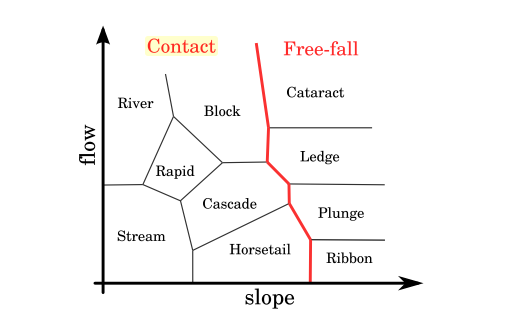
\includegraphics[]{waterfall_classification.png}
	\caption{Waterfall classifications \cite{Emilien2014}}
\end{figure}

\subsection{Simulation-based}

Simulation-based techniques attempt to reproduce real-world phenomena to determine river networks on given terrains. These simulations vary greatly in the level of detail they attempt to reproduce and can be split into the following sub-categories which will be discussed in further detail below: \textit{Gravitation simulation} \textit{Erosion-simulation}, \textit{Rainfall simulation} \\

\subsubsection{Gravity-simulation}

Gravity simulation techniques attempt to determine the path water will take on the terrain by simulating the effects of gravity. \\

In order to generate plausible rivers, Belhadg et Audibert \cite{Belhadj2005} simulate the effect gravity has on water particles placed on the peaks of pre-generated ridges. To create the ridges, particle pairs are first placed at random locations on the terrain. These particle pairs are then randomly assigned an axis and iteratively, both particles distance themselves in opposite directions, perpendicular to this axis. At each iteration a new vertex is placed and its height calculated based on a Gaussian distribution. To create the river networks, river particles are placed on the top of these generated ridges and a simple physical simulation which takes into consideration particle velocity, particle mass and surface friction is used to model the motion of these particles on the terrain. The path followed by these particles is tracked and, when two paths intersect, their particle velocity and mass are combined. When all particles have stopped moving the simulation is deemed balanced and all particle paths which do not lead to terrain extremities are discarded. The remaining particle paths are kept and form the core river network. To initialise the remaining vertices on the terrain, interpolation is performed based on the height of surrounding river and ridge vertices.\\

Similarly, in the work by Soon Tee \cite{Teoh2008}, water is placed at specific locations on the terrain either by the user or whilst simulating rainfall. To determine the water course on the terrain, the surrounding vertex with lowest height is iteratively followed until a local minima is found or the terrain extremities is reached.\\

In their work on modelling the effects of hydraulic erosion, Št'Ava et al. \cite{StAva2008} first need to determine the course the water takes on the terrain. To do so, the terrain is split into equal-sized (configurable) columns and a hydrostatic pipe-model simulation is used to evacuate water from source to surrounding destination columns iteratively. Column heights, fluid density and gravitational acceleration directly influences the inter-column water transfers. \\

\subsubsection{Erosion-simulation}

Erosion-based simulations attempt to produce realistic terrains by modelling the effect of erosion. Erosion is a direct consequence of exogenic processes (water flow, wind, temperature) and is characterised by the removal of soil and rock from one location on earth's surface to be redeposited on another. Earth's landscape is a direct consequence of erosion and reproducing this phenomena accurately is core to procedurally generating accurate landscapes. Both Kelly et al. \cite{Kelley1988} and Št'Ava et al. \cite{StAva2008} attempt to produce plausible terrains by modelling the effects of erosion.\\

In the work by Kelley et al. \cite{Kelley1988}, the user specifies, on a horizontal plane, the terrain outline along with the main trunk stream. The terrain outline is used to configure the terrain extremities once ported to a 3 dimensional space. The main trunk stream specifies the path which the highest order water stream should follow on the resulting terrain. Given this terrain outline and the position of the initial main trunk stream, the system iteratively increments the number of nodes which form the main trunk in order to add streams to the network. The number of new nodes added depends on the drainage area (surface area that a stream needs to channel) and the soil type as more resistant soil materials (e.g. stone) will be less influenced by water erosion than weaker ones (e.g. clay). \\

Št'Ava et al. \cite{StAva2008} are able to simulate the effects of hydraulic erosion on a terrain in real-time by using the massively parallel architectures of GPUs. Virtual pipettes are used by the user to drop water at required locations on the terrain and a gravitation simulation mentioned above is used to determine the base water course on the terrain. Whilst the water is being routed through the terrain \textit{force-based} and \textit{dissolution-based} erosion is simulated. \textit{Force-based} erosion is a direct consequence of the the force of the water on the terrain surface (figure \ref{force-based erosion}. Dissolution-based erosion is a consequence of the water mass on the terrain surface under the water and is most often characterised by a smoothing effect.\\

\begin{figure}[h]
  \centering
	\label{force-based erosion}
	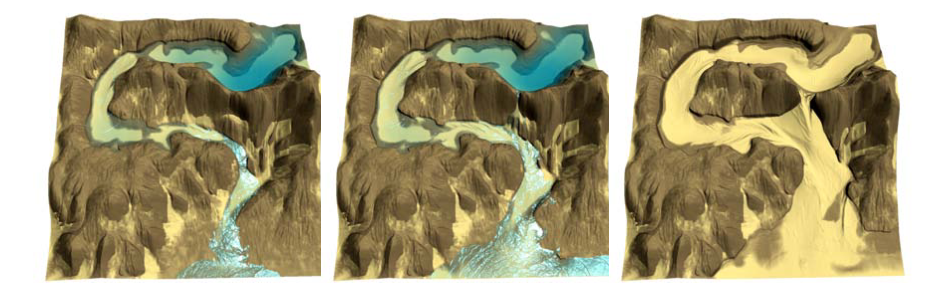
\includegraphics[]{force_based_erosion.png}
	\caption{Simulation of the effect of force-based erosion caused by running water \cite{StAva2008}}
\end{figure}

\begin{figure}[h]
  \centering
	\label{dissolution_based_erosion-based erosion}
	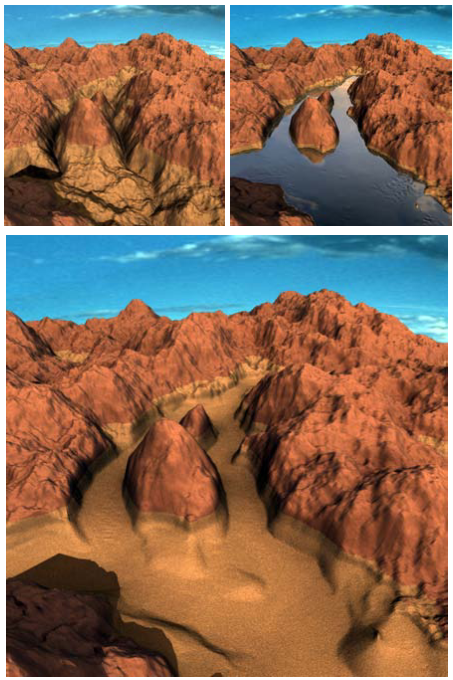
\includegraphics[]{dissolution_based_erosion.png}
	\caption{Simulation of dissolution-based erosion erosion caused by water movement\cite{StAva2008}}
\end{figure}

\subsubsection{Rainfall simulations}

In order to determine where on the terrain rivers will appear, work by Soon Tee \cite{Teoh2008} performs a rainfall simulation to determine both the location and quantity of water at different points on the terrain followed by a gravitation simulation (mentioned above) to determine the course of the water on the terrain. The rainfall simulation requires the user to specify wind direction and maximum rainfall. Then, starting from the source of the wind, the system simulates clouds moving in the direction of the wind with a configured velocity. When contact is made with points on the terrain, water is dropped on the corresponding cell. The amount of water dropped increases with altitude and zeroes out when all available rainfall is depleted. 

\\-------------------------------------------

\textit{Fractal-based} techniques use recursive splitting and string rewriting similar to L-systems to determine a plausible path for a river to follow.\\

Derzapf ET AL. --> RIVER NETWORKS FOR INSTANT PROCEDURAL PLANETS

c: Heuristic

TERRAIN ADAPTS TO RIVER

In their work, Derzapf et al. permit the creation of procedural planets at any scale in real-time. To do so, only a rough representation of the planet is generated and detailed content is produced on-the-fly when the user navigates through it. This has the advantage of keeping memory usage minimum whilst not compromising on realism. To ensure updates are performed in real-time, their algorithms are implemented to take use of the massively parallel architecture of GPUs. \\
To initialise high-level planets, the system first creates the base mesh with all contained vertices representing the sea. The system then selects a given number of seed continent vertices and allows them to spread until a user-configured land-to-water ratio is reached. At this point, the "rough" planet is a mesh with each vertex assigned one of two labels: continent or sea.\\
To create the rivers the system iterates through all continental vertices in pseudo-random order to find those that are adjacent to a sea vertex. When such a vertex is found, it acts as the river mouth from which adjacent continental vertices chosen pseudo-randomly are connected. This is performed iteratively to form the river networks.\\
To assign ground altitudes to the river vertices the system employs the following formula for each river vertex, starting from the river mouth:

$a_{v} = a_{u} + e_{a}l_{e}\xi , e_{a} = \frac{a_{max_river}}{l_{r}} $

Where:
\begin{itemize}
\item $a_{v}$ is the ground altitude of the current vertex.
\item $a_{u}$ is the ground altitude of the previously processed vertex (or zero if \textit{v} is the first vertex).
\item $e_{a}$ is the average ground elevation.
\item $l_{e}$ is the length of the current vertex.
\item $\xi \in [0,1[$ is a uniformly distributed pseudo-random number.
\item $a_{max_river}$ is the user-configured maximum river altitude.
\item $l_{r}$ is the current river length.
\end{itemize}

When the ground altitudes have been assigned, the following formula is used iteratively on each river vertex to assign water altitudes:

$w_{v} = a_{v} + e_{w}l_{e}, e_{w} = \frac{\epsilon_{river}}{l_{cr}} $

Where:
\begin{itemize}
\item $w_{v}$ is the water altitude of the current vertex.
\item $a_{v}$ is the ground altitude of the current vertex.
\item $e_{w}$ is the average water elevation.
\item $l_{e}$ is the length of the current vertex.
\item $\epsilon_{river}$ is the maximum river depth.
\item $l_{cr}$ is the distance from the current vertex to the river spring.
\end{itemize}

Once this has been performed, the "rough terrain" is comprised of continental vertices, river vertices and sea vertices, each with a defined altitude.\\

All randomness in the algorithms depends on a configured seed value, enabling virtual virtual worlds to be easily reproducible. This has the added advantage of permitting networked users to explore the same virtual world with very little data exchange. \\


SMELIK ET AL. --> INTERACTIVE CREATION OF VIRTUAL WORLDS USING PROCEDURAL SKETCHING

c: Explicit

RIVER ADAPTS TO TERRAIN, EXPLICIT USER CONTROL

In their work, Smelik et al. create an interactive system which permits users to model a complete virtual world with content ranging from rural features (mountains, rivers, etc.) to man-made ones (buildings, road networks). In order to promote user-intuitiveness, they focus strongly on user controls and develop novel interaction tools which include sketch recognition.\\
When modelling the virtual world, interactions are split into two modes: \textbf{Landscape} and \textbf{Feature}. \textit{Landscape mode} permits the designer to paint ecotopes onto the terrain using traditional image editing tools. These ecotopes are predefined by the user and encompass both elevation and soil material information. In \textit{feature mode}, the user is able to place terrain content which include rivers. To place these rivers, the user must sketch vector lines outlining the core path of the river. Based on this information, a suitable course is plotted through the landscape, river banks inserted and other terrain features to which the river takes precedence adapted. For example, if the river is plotted to pass through a forest, trees on the rived bed and bank will be removed. 


Pmsinkiewicz ET AL. --> A fractal model of mountains and rivers
Musgrave et al. --> The synthesis and rendering of eroded fractal terrains | Also fractal 

TERRAIN ADAPTS TO RIVER

C: Fractal

In their work, Pmsinkiewicz et al. use an adapted midpoint-displacement technique to procedurally generate plausible rivers on terrain. Midpoint-displacement is a fractal technique heavily used for the creation of realistic looking terrain height-maps. Given a starting triangle representing the terrain, \textit{A}, midpoint-displacement iteratively subdivides \textit{A} into four smaller triangles. Each time new triangle vertices are created they are displaced vertically by a random offset. This process is repeated until a given recursion limit is reached. See figure \ref{Midpoint displacement} for an example of a single iteration of the process.

\begin{figure}[h]
  \centering
	\label{Midpoint displacement}
	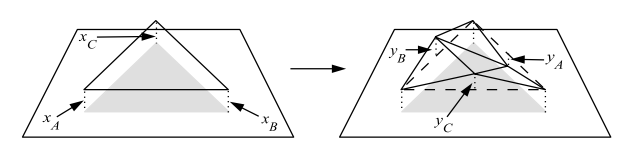
\includegraphics[width=\textwidth]{midpoint_displacement.png}
	\caption{A single iteration of midpoint displacement for the creation of mountains \cite{Prusinkiewicz1993}. New vertices $y_{A}$, $y_{B}$ and $y_{C}$ are created and shifted vertically by a random offset}
\end{figure}

To adapt this method to the generation of rivers on the terrain, the edges of each newly formed triangle are labelled as \textit{entry}, \textit{exit} or \textit{neutral}. An entry edge defines the point of entry for the river into the triangle, an exit edge the point of exit and a neutral edge prevents the river from passing through.\\

When a production step is applied and a triangle split, the following constraints must be applied:
\begin{itemize}
\item An entry edge must split into an entry and a neutral edge.
\item An exit edge must split into an exit edge and a neutral edge.
\item A neutral edge must split into two neutral edges.
\item The newly formed edge-pairs within the triangle must either be "entry/exit" or "neutral/neutral".
\end{itemize}

See figure \ref{Single production of midpoint displacement adapted to river generation. Given the initial triangle, four valid split scenarios. } for example valid productions.

\begin{figure}[h]
  \centering
	\label{Single production of midpoint displacement adapted to river generation. Given the initial triangle, four valid split scenarios. }
	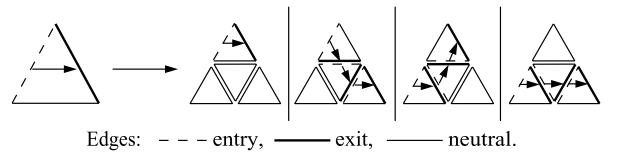
\includegraphics[width=\textwidth]{midpoint_displacement_for_rivers_1.png}
	\caption{Single production of midpoint displacement adapted to river generation \cite{Prusinkiewicz1993}. Given the initial triangle, four valid split scenarios.}
\end{figure}

One difficulty with this technique is to ensure two adjacent triangles are coherent once they split. That is, that the exit edge of one coincides with the entry edge of the other edge. To overcome this, the location of the vertices of an edge are used as the key to a random number generating hash table which, depending on its output, determines which segment will be crossed by the river.\\
When complete, a river path which is guaranteed not to cross itself is created. Post-processing is then used to create realistic terrain surrounding the riverbed.



Teoh, Soon Tee --> River and coastal action in automatic terrain generation

RIVER ADAPTED TO TERRAIN

c: Explicit & Simulation

The work by Soon Tee \cite{Teoh2008} permit the procedural generation of terrains, river meanders, river deltas, coastal cliffs and coastal beaches. Similarly to the work by Belhadg et Audibert \cite{Belhadj2005}, the user starts by creating ridges and mountain ranges that form the base terrain. When this is done, the user is able to place seas, lakes and rivers.\\
Two methods can be used to place water reserves (lakes and seas) in their system: \textit{flood filling} and \textit{locating substantial local minima}.\\ \textit{Flood filling} is a commonly used technique to place water on terrains and requires the user to click a point on the terrain which will act as the seed point for the water surface. This seed will then propagate iteratively to surrounding points which are at a lower height until there are no more lower points to propagate to.\\
With \textit{locating substantial local minima}, the system automatically detects locations on the terrain which are local minimums and could therefore cater a lake or a sea. The user can then raise the surface height manually. \\
To place rivers on the terrain the user can either explicitly point out the start of the stream or the system can generate them by performing a simulation based on total rainfall, wind direction and terrain relief. To explicitly point out the start of the stream, the user must simply click the relevant point on the terrain. A simplified model of gravity is subsequently used where the water is iteratively evacuated to its lowest surrounding point. This process finishes and the river deemed complete when the path reaches a local minima or terrain borders.\\
The simulation approach requires the user to specify wind direction and maximum rainfall. Then, starting from the source of the wind, the system simulates clouds moving in the direction of the wind with precipitation increasing with altitude until all rainfall has been depleted. The path taken by the rain and consequentially the rivers, is then determined similarly to the method mentioned previously for explicit river instantiation. 

Génevaux et al. --> Terrain generation using procedural models based on hydrology

c: Fractal and Classification-based

Génevaux et al. \cite{Genevaux2013} permit users to procedurally generate terrains based on models of hydrology. To so, the user first sketches the contour of the terrain and optionally some river paths within the terrain and output nodes on the contour which will represent the river mouth. If no candidate output nodes are specified by the user, they are determined heuristically from geomorphology data based on the shape of the contour.\\
These seed nodes are then iteratively expanded to form a larger network of rivers. To do so, on each iteration a candidate node is selected for expansion based on elevation and priority. The weighting between elevation and priority is configured by the user and has a large effect on the resulting river network. For example, by prioritising candidate nodes at lower elevations, lowlands will be generated first.\\
Rewriting grammar is used to perform node expansion. Configured values of $\rho_{a}, \rho_{s} and \rho_{c}$ influence the probability of selecting production rules favouring asymmetric branching, symmetric branching and continuation without branching respectively. The position for the new node is then selected using the following constraints:
\begin{itemize}
\item It should be at a minimum distance from existing nodes and edges.
\item The new node should be at a greater distance from the terrain contour.
\item The new node should be compatible with the elevation constraints of existing nodes.
\end{itemize}
If a position satisfying these constraints is found, a new node is added at the given position and the process is repeated.\\
The system then creates Voronoi cells centered around the river network nodes. Cells belonging to individual watersheds are then concatenated and plausible heights are generated for all points within those cells in order to keep the river flowing downwards at all times. Based on the calculated flow intensity (slope dependant), water drainage and soil type, appropriate rivers are then placed.
